\documentclass[notes, dvipsnames]{beamer}

\usepackage{default}
\usepackage[dutch]{babel}
\usepackage{pgfpages}
\usepackage{pgf-pie}
\usepackage{ifthen}
\usepackage{qtree}
\usepackage[utf8]{inputenc}

\usetheme{Frankfurt}
\usecolortheme{beaver}
\setbeamertemplate{note page}{\pagecolor{yellow!25}\insertnote}
\setbeamertemplate{note page}{\pagecolor{white}\insertnote}

\title{Automatisch vertalen van logigrammen naar een getypeerde logica}
\subtitle{Thesisverdediging}

\author{Jens Claes}
\date{28 juni 2017}

\newcommand{\seperation}{
	\vspace{1em}
	\ppause
}
\newcommand{\sseperation}{
	\vspace{1em}
}
\newcommand{\hitem}{
	\ppause
	\item
}
\newcommand{\ppause}{\onslide<+>}
\newcommand{\nnote}[1]{\note<.>{#1}}
\setbeamercovered{%
	still covered={\opaqueness<1->{0}},
	again covered={\opaqueness<1->{60}}
}
\setbeameroption{hide notes} % Only slides
% \setbeameroption{show notes on second screen=right} % Both

\newcommand{\attention}[1]{\textcolor{ForestGreen}{#1}}

%\graphicspath{ {../images/} }

\setbeamertemplate{bibliography item}{\insertbiblabel}
\AtBeginSection[]
{
   \begin{frame}
        \frametitle{Inhoudstafel}
        \tableofcontents[ 
              currentsection,
              hideothersubsections
            ] 
   \end{frame}
}
\begin{document}
	\frame{\titlepage}

  \begin{frame}
    \frametitle{Inhoudstafel}
    \tableofcontents[hidesubsections] 
    \nnote{
      \item Inleiding tot domein waarbinnen het probleem zich afspeelt
      \item Concrete probleemstelling
      \item Systeem oplossing probleem
      \item Evaluatie Systeem
    }
  \end{frame}

  \section{Inleiding}
	\begin{frame}{Knowledge Base Systems}
		\begin{itemize}
      \hitem Invoer: Kennisbank
      \item Specificatie van de wereld
      \nnote{
        \item Kennisbank is invoer systeem. Bestaat uit vocabularium (waarover) en theorie (wat, regels)
        \item Bijvoorbeeld geen 2 thesisverdedigingen in 1 lokaal
        \item Bijvoorbeeld geen 2 deuren tegelijk open (dubbele deur bank)
      }

			\seperation
      \item Inferenties \cite{idp}
        \nnote{
          \item Bron: De cat en al (scheduling)
          \item Programma's op die kennisbank
          \item geen domeinkennis
          \item toepasbaar op verschillende specificaties
        }
        \begin{itemize}
          \hitem Propagatie \nnote{ISP: Automatisch Selecteren volgtijdelijkheidsvoorwaarden na selecteren vervolgvak}
          \hitem Model expansie \nnote{ISP: Genereren volledig ISP vanuit partieel rooster}
          \hitem Bevraging \nnote{Opvragen individueel uurrooster}
        \end{itemize}

      \seperation
      \item Kennisrepresentatietaal
      \nnote{
        \item Om kennis voor te stellen
        \item Bijvoorbeeld eerste orde logica, maar ook uitbreiding: types, modale logica, ...
        \item Moeilijk om te lezen, schrijven en leren
      }
		\end{itemize}
	\end{frame}

	\begin{frame}{Controlled Natural Language (CNL)}
		\begin{itemize}
      \hitem Gecontroleerde natuurlijke taal
      \item Subset natuurlijke taal
      \nnote{
        NAAST KBS
        \item Enkel bepaalde zinsconstructies toestaan
      }

      \seperation
      \item Makkelijker te schrijven/lezen
      \nnote{
        \item Doel: makkelijker schrijven/lezen
        \item Consistenter
      }
      \hitem Formele semantiek
      \nnote{
        \item Sommige formele semantiek
        \item Bruikbaar als kennisrepresentatietaal (ook gedaan)
        \item Slecht gedocumenteerde semantiek
      }
		\end{itemize}
	\end{frame}

	\section{Probleem}
	\begin{frame}{Probleemstelling}
		\begin{itemize}
      \hitem Kennisrepresentatietaal
        \begin{itemize}
          \item Toegankelijk
          \item Rijk genoeg
          \item Toepasbaar binnen KBS
        \end{itemize}
        \nnote{
          \item Ontwikkelen van nieuwe kennisrepresentatietaal die aan eisen voldoet
          \item Onderzoeken CNL
          \item Beter gedocumenteerde vertaling
          \item Uitbreiden van CNL met types
        }

      \seperation
      \item Extra: types
      \nnote{
        ``Het huis drinkt het gras''
        \item Vertalen naar getypeerde logica
        \item Extra inferentie op basis van types: later meer
      }

      \seperation
      \item Logigrammen (uit \cite{logigrammen})
        \nnote{
          \item Talrijk, klein en simpele logica: handige eerste test
          \item Nog niet ``rijk genoeg'' maar wel ``toegankelijk'' en ``toepasbaar binnen KBS''
        }
		\end{itemize}
	\end{frame}

	\begin{frame}{Logigrammen}
    \begin{figure}
      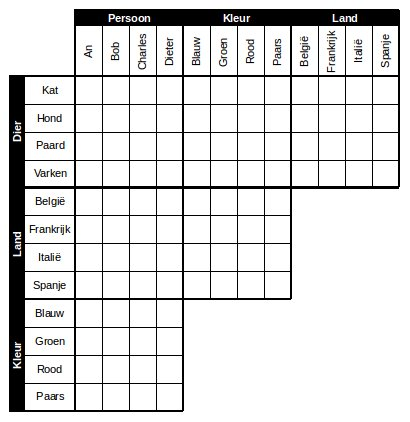
\includegraphics[width=0.6\textwidth]{logigram.jpg}
    \end{figure}
    \note{
        \item Kader + aantal zinnen in natuurlijke taal: clues

        \sseperation
        \sseperation
        \item Aantal domeinen (nationaliteiten, dieren, kleuren, ...)
        \item Aantal domeinelementen (Noor, Brit, kat, hond, ...)
        \item 1 bijectie tussen elk paar domeinen
        \item Zinnen: constraints op die bijecties
        \item Doel: Zoek de waarde van de bijecties

        \sseperation
        \sseperation
        \item Redelijke uniforme zinstructuur
        \item Geschikt om automatisch om te zetten naar logica
    }
	\end{frame}

	\begin{frame}{Inferenties op logigrammen}
		\begin{itemize}
      \ppause
      \nnote{
        Toepasbaar binnen KBS: inferenties op specificatie van logigram mogelijk
      }
      \hitem Oplossen
      \nnote{
        Gegeven clues, puzzel oplossen. Enige inferentie die wij hebben gedaan
      }
      \hitem Status clues
      \nnote{
        gegeven clues + partiele oplossing, onderverdeling in 3 groepen. Bijvoorbeeld ``John heeft een kat''
        \item Clues die altijd voldaan zijn in uitbreiding van oplossing: niet meer nodig (John heeft een kat in model)
        \item Clues die voldaan zijn in sommige uitbreidingen maar niet in allemaal: nuttige informatie (John heeft niets in model)
        \item Clues die nooit voldaan zijn in uitbreiding van oplossing: partiele oplossing is fout (John heeft een hond in model)
      }
      \hitem Hint
      \nnote{
        Gegeven partiële oplossing, geef subset clues die samen voor propagatie kunnen zorgen
        \item Gebruiker niet alle hints afgaan
      }
      \hitem Schrijfhulp
      \nnote{
        Gegeven clues: geef mogelijke oplossingen
        \item auteur kan zorgen dat er een deel geschrapt worden
        \item Of: Duid overbodige zinnen aan
      }
		\end{itemize}
	\end{frame}
	
	\section{Systeem}
  % \subsection{Overzicht}
	\begin{frame}{Systeem Thesis}
		\begin{enumerate}
      \hitem Vertaal + leid types af
      \nnote{
        De eerste stap is de grootste
        \item vertaling via framework
        \item types via (eigen) uitbreiding framework
        \item Invoer: probleem-specifiek lexicon + clues, dat is alles!
        \item Theorie (formele vertaling zinnen) + type-informatie
      }
      \hitem Infereer domeinen
      \nnote{
        uit type-informatie
        \item Interactie met gebruiker mogelijk
      }
      \hitem Formeel vocabularium
      \nnote{
        uit domeinen logigram
        \item Waarover logigram gaat
      }
      \hitem Axioma's
      \nnote{
        Extra zinnen voor de theorie die impliciet zijn aan logigram
        \item op basis van type-informatie
      }
      \hitem Pas inferentie toe
      \nnote{
        Wij beperkt tot ``oplossen'' maar we hebben volledige specificatie dus andere ook mogelijk
        \item geen onderzoek naar inferenties op logigrammen
      }
		\end{enumerate}
	\end{frame}

  % \subsection{Framework}
	\begin{frame}{Framework}
		\begin{itemize}
      \hitem Blackburn en Bos \cite{Blackburn2005, Blackburn2006}
      \nnote{Goed gedocumenteerd: 2 boeken over}

      \seperation
      \item Compositioneel
      \item $\lambda$-calculus
      \item Semantiek in lexicon
      \nnote{
        Betekenis zit in woorden (lambda-formules)
        \item Via Frege's compositionaliteits principe naar betekenis woordgroepen + zinnen
      }
      \hitem 4 onderdelen
      \nnote{
        4 onderdelen staan los van elkaar
        \begin{itemize}
          \item Lexicon/Vocabularium: per probleem, taalkundige categorieën
          \item Grammatica: contextvrij, categorial combinatorial grammar (Baral et al. \cite{Baral2008}), ...
          \item Lexicale semantiek: per taalkundige categorie betekenis (semantisce macro's); eerste-orde logica, discourse representation structures, event-based logic, ...
          \item Grammaticale semantiek: gekoppeld aan grammatica en lexicale semantiek; rule-to-rule correspondence: syntactische regel leidt tot semantische regel
        \end{itemize}
      }

      \seperation
      \item Aangepast voor logigrammen
      \nnote{
        \item Lexicon: enkel existentiële kwantificatie
        \item valsspelen: eigennamen, ...
        \item predicaten: werkwoorden en voorzetsels
        \item Algemene en specifieke grammaticale regels
        \item Alldifferent, simpele arithmetiek
        \item Toevoegen types
      }
		\end{itemize}
	\end{frame}

  % \subsection{Types}
	\begin{frame}{Types}
    \begin{itemize}
      \hitem Het huis drinkt de tuin

      \seperation
      \item Via taalkundige ``features''
      \nnote{
        Bv. $NP[num]$ meervoud of enkelvoud
      }

      \seperation
      \item Simpel typesysteem
      \nnote{
        \item basistypes + pair-types voor werkwoorden en voorzetsels
        \item $NP[type]$: één van de domeinen
        \item $TV[type]$: paar van twee domeinen
      }
    \end{itemize}
	\end{frame}

  \begin{frame}{Inferentie Domeinen}
    \begin{itemize}
      \hitem Type-inferentie
      \item Type uniek per woord
      \nnote{
        Uitbreiding: lexicon geannoteerd met types
        \item WIJ laten annotaties weg: zullen het infereren
        \item veronderstelling: uniek type
        \item NIET AAN VOLDAAN!
        \item Opdeling van woorden in domeinen
      }
      \hitem Taalkundige vragen gebruiker
      \nnote{
        \item Omwille van synoniemen niet altijd helemaal mogelijk
        \item Mogelijke vragen: Synoniemen, mogelijk lijdend voorwerp, 2 woorden zelfde type?
      }
    \end{itemize}
  \end{frame}

  \begin{frame}{Een complete specificatie}
    \begin{itemize}
      \ppause
      \nnote{
        Naast theorie uit vertaling clues, nog dingen nodig voor volledige specificatie
      }
      \hitem Formeel vocabularium
      \nnote{
        \item Afgeleid uit types
        \item Domeinen = Constructed Type (DCA, UNA)
        \item Getallen = Subsets
        \item Andere types ``John follows the tour with 54 people'' ook constructed types
      }
      \hitem Axioma's
      \nnote{
        Logigram-specifieke axioma's
      }
      \begin{itemize}
        \hitem Bijectie
        \nnote{
          Elk predicaat is een bijectie (veronderstelling logigram)
        }
        \hitem Symmetriebrekers
        \nnote{
          tourA $\to$ The tour with 54 people, tourB $\to$ the tour with 44 people, ...
        }
        \hitem Synoniemen
        \nnote{
          Zelfde signatuur? Zelfde predicaat!
        }
        \hitem Equivalentierelatie (transitief, symmetrisch)
        \nnote{
          Equivalentieklassen is wat we zoeken
          \item 2 domeinelementen equivalent als ze gebonden via predicaat
          \item Equivalentie-axioma's op basis van types van predicaten
        }
      \end{itemize}
    \end{itemize}
  \end{frame}

  \section{Evaluatie}
  \begin{frame}{Evaluatie}
    \begin{itemize}
      \hitem Puzzle Baron's Logic Puzzles Volume 3 \cite{logigrammen}
      \nnote{
        \item Training = eerste 10
        \item Test = volgende 10
      }

      \seperation
      \item Kleine aanpassingen
      \item Automatisch oplosbaar
      \nnote{
        \item 2 zinnen met grote(re) aanpassing
        \item In 2 logigrammen vragen van type 4: slecht type-systeem
        \item In 3 logigrammen geen vragen
      }
    \end{itemize}
  \end{frame}

  \begin{frame}{Evaluatie}
    \begin{table}[t]
      \centering
      \begin{tabular}{lc}
        \hline
        \textbf{Probleem} & \textbf{Aantal voorkomens} \\ 
        \hline
        ``the one'' & 15 \\
        Ongezien gebruik koppelwerkwoord & 6 \\
        Slecht gestructureerde bijzin & 6 \\
        Passieve zin & 1 \\
        Bezittelijk voornaamwoord & 1 \\
        Slecht gestructureerde naamwoordgroep & 1 \\
        \hline
        Gehele getallen & 3 \\
        Superlatief & 1 \\
        ``Of the two ...'' & 1 \\
        \hline
        Slecht getypeerd werkwoord & 14 \\
        Slecht getypeerde naamwoordgroep & 5 \\
        \hline
        Meer dan één woordvorm eigennaam  & 1 \\
        \hline
        Overbodig woord & 7 \\
        Ontbrekend woord (ellips) & 3 \\
        \hline
      \end{tabular}
      \caption{Een overzicht van de aanpassingen}
      \label{tbl:resultaten}
    \end{table}
    \note{
      \item Groep 1: 30/65 nieuwe grammaticale elementen
      \item Groep 2: 5/65 gelijkaardig aan training-set
      \item Groep 3: 19/65 slecht type-systeem
      \item Groep 4: 1/65 Foute assumptie eigennaam uniek
      \item Groep 5: 10 kleine woordjes te veel of te weinig (niet essentie van de zin)
    }
  \end{frame}

  \section{Conclusie}
  \begin{frame}{Conclusie}
    \begin{itemize}
      \hitem Goed framework
      \nnote{
        Voor CNL met formele semantiek
        \item Goed gedocumenteerd
        \item Duidelijke scheiding 4 onderdelen (engineering practice)
      }
      \hitem Inferentie op CNL mogelijk
      \nnote{
        \item Enkel ``oplossen'' uitgewerkt maar specificatie is er dus de rest kan ook
        \item (niet nieuw, ook al voor ACE en PENG)
        \item Toegankelijke taal (min of meer uit boekje) is toepasbaar binnen KBS
        \item ze is ook rijk genoeg (wel geen superlatieven)
      }
      \hitem Getypeerde CNL
      \nnote{
        \item Nu type-inferentie + getypeerde logica, meer is mogelijk, ook moeilijker type-systeem
        \item e.g. to order food or drinks (multiple types per woord)
        \item Verbeterde schrijftools voor CNL's ?
      }
    \end{itemize}
  \end{frame}

			
	\section{Referenties}
	\begin{frame}[allowframebreaks]{Referenties}
		\bibliographystyle{plain}
		\bibliography{../thesis/referenties}
	\end{frame}
	
\end{document}
